
\documentclass{beamer}

\usepackage{algpseudocode, color, colortbl, listings, MnSymbol}

\usepackage{hyperref}
\hypersetup{
    colorlinks=true,
    urlcolor=blue,
}

\usetheme{Montpellier}
\usecolortheme{rose}

% page numbers, from
% https://tex.stackexchange.com/questions/137022/how-to-insert-page-number-in-beamer-navigation-symbols
\expandafter\def\expandafter\insertshorttitle\expandafter{%
  \insertshorttitle\hfill%
  \insertframenumber\,/\,\inserttotalframenumber}

\definecolor{Gray}{gray}{0.8}
\newcolumntype{g}{>{\columncolor{Gray}}c}

\newcommand{\stanza}{ \\~\ }

\title{11. Convex Hull and Closest Pair}
\subtitle{CPSC 535 $\sim$ Spring 2019}
\author{Kevin A. Wortman}
\institute{ 
\includegraphics[height=2cm]{csuf-logo-cmyk} }
\date{April 29, 2019 \stanza

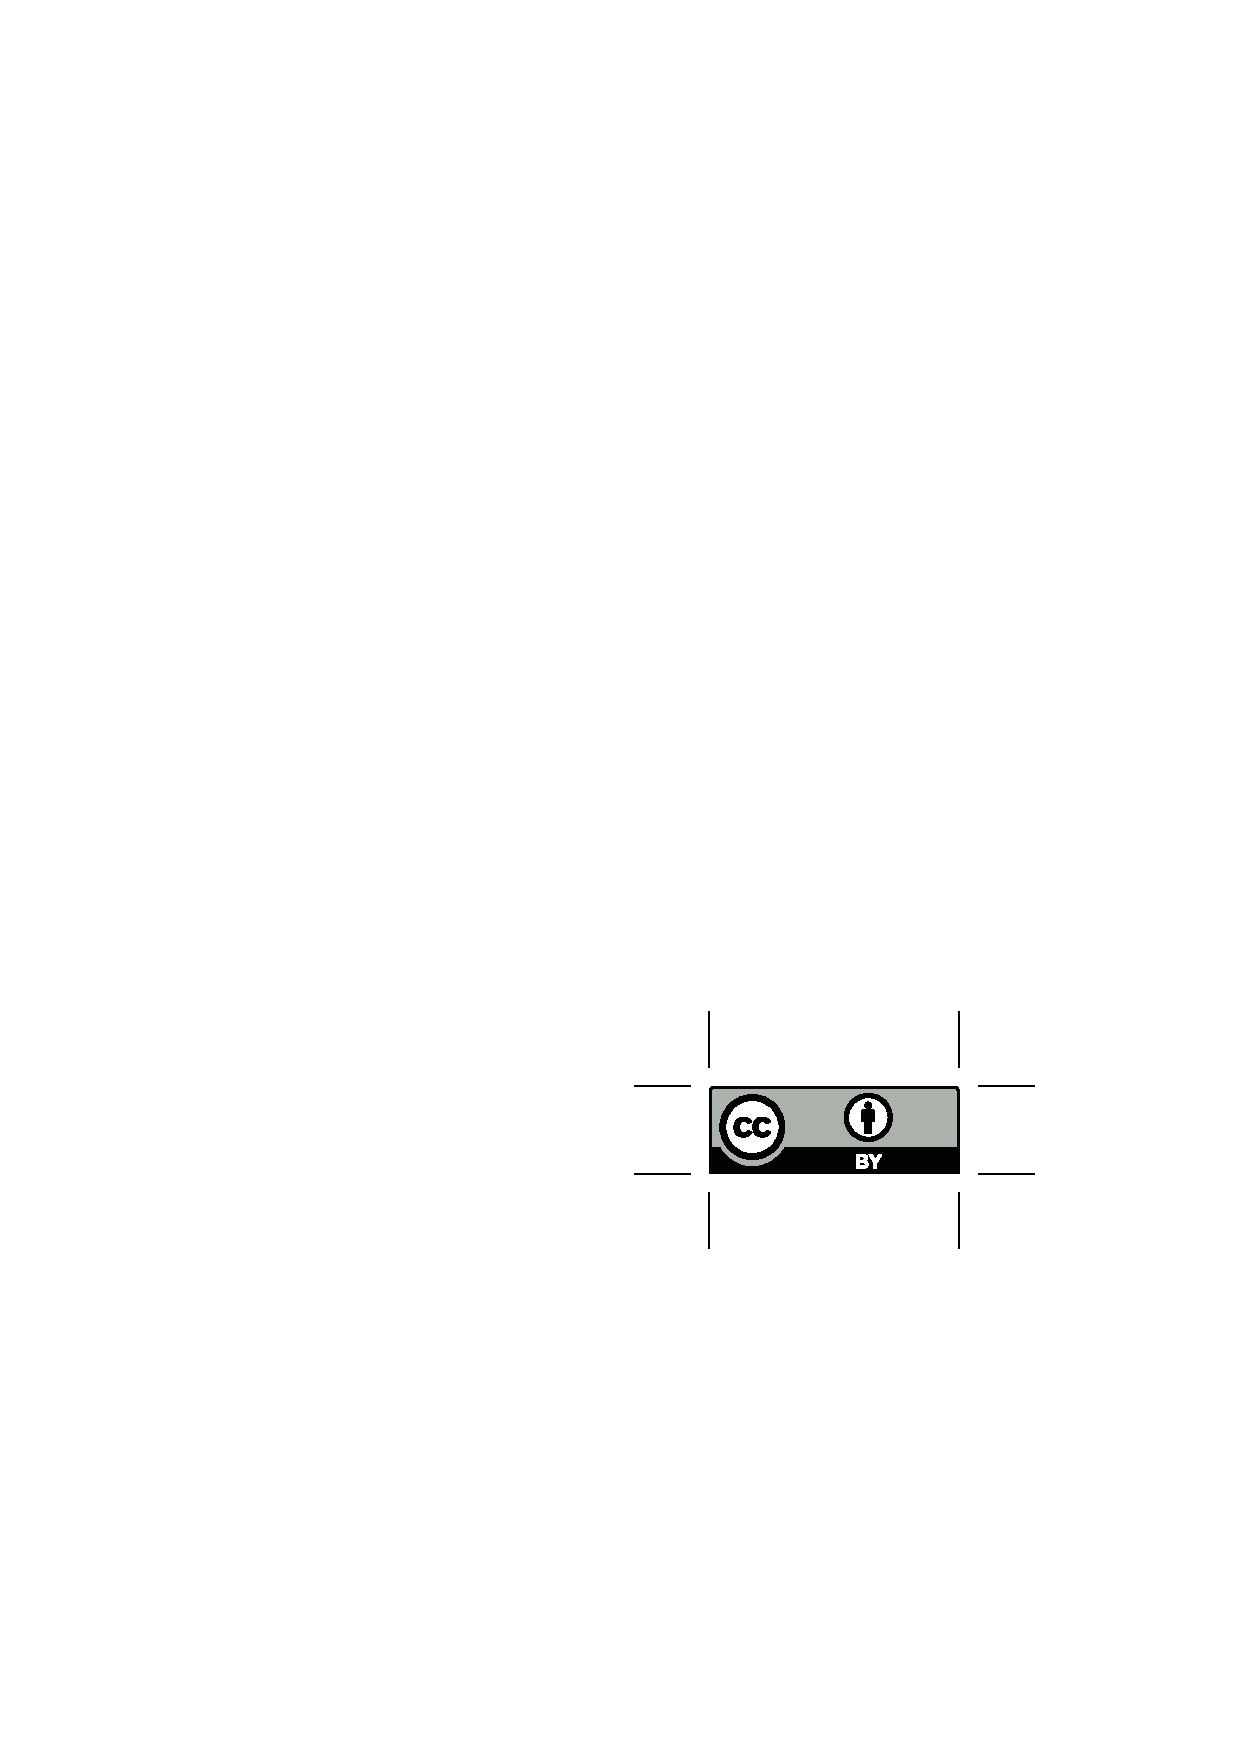
\includegraphics[height=14pt]{by} \\

{\tiny
This work is licensed under a
\href{http://creativecommons.org/licenses/by/4.0/}{Creative Commons Attribution 4.0 International License}.
}}

\begin{document}

\begin{frame}
  \titlepage
\end{frame}

\begin{frame} \frametitle{Convex Hulls}
\emph{convex hull problem} \\
\textbf{input}: set of $n \geq 3$ points $Q$ \\
\textbf{output}: $CH(Q)$, the subset of $Q$ that is the set of vertices on
  the convex hull of $Q$ \stanza

Convex hull $\equiv$ boundary of convex polygon enclosing all of $Q$ \stanza

Applications
\begin{itemize}
  \item object intersection in raytracing, video games, GUIs
  \item drawing implicit regions in GIS
  \item finding farthest points
  \item component of other algorithms
\end{itemize}
\end{frame}

\begin{frame} \frametitle{Approaches to Convex Hulls}
Like the sorting problem, many algorithm patterns work for convex hulls,
and there is a rich literature of competitive algorithms. \stanza

\begin{itemize}
  \item Greedy pattern: line-sweep, update hull as we go
  \item Divide-and-conquer: divide $Q$ in half, compute convex hulls for each
    half, merge two convex hulls into one
  \item Iterative improvement: start with a superset of $CH(Q)$; refine by repeatedly eliminating
    a constant fraction of the points until only $CH(Q)$ remains
\end{itemize}
\end{frame}

\begin{frame} \frametitle{Baseline Algorithm}
\textbf{Observe}
\begin{itemize}
  \item any two input points define a line $\ell$
  \item when those points are both in $CH(Q),$ remaining $n-2$ points are all on
    the same side of $\ell$ \emph{(geometric property)}
  \item $\implies$ for each pair of input points $p, q$, see whether all other points
    are on the same side of $\ell$
  \item if so include $p, q$ in $CH(Q)$
\end{itemize}
\end{frame}

\begin{frame} \frametitle{Baseline Pseudocode}
  {\small
\begin{algorithmic}[1]
  \Function{NAIVE-CONVEX-HULL}{$Q$}
    \State $H=\emptyset$
    \For { distinct points $p, q \in Q$ }
      \State form line $\ell$ intersecting $p$ and $q$
      \State $k = $ \# points above $\ell$
      \If { $k=(n-2)$ or $k=0$ }
        \State $H = H \cup \{p, q\}$
      \EndIf
    \EndFor
    \State \Return $H$
  \EndFunction
\end{algorithmic}
}

\textbf{Analysis}: $\Theta(n^3)$ time
\end{frame}

\begin{frame} \frametitle{Graham Scan Idea}
\begin{itemize}
  \item greedy pattern, reduction-to-sorting
  \item Heuristic: when touring the hull in counter-clockwise order, we
    \textbf{only make left turns}
  \item right turn $=$ exiting a concavity
  \item $\therefore$ sweep counter-clockwise, keep points that participate in left
    turns, drop points that cause right turns
  \item alternative kind of line sweep: rotating the line (not left-to-right)
\end{itemize}
\end{frame}

\begin{frame} \frametitle{Graham Scan Greedy Heuristic}
\begin{itemize}
  \item $p_1, \ldots, p_m = Q$ sorted into counter-clockwise order, eliminating ties
  \item stack $S$ of points; contains hull of points visited \emph{already}
  \item base case: push first 3 points onto $S$
  \begin{itemize}
    \item for any three points $p, q, r$ forming a non-degenerate triangle,
      $CH(\{p, q, r\}) = \{p, q, r\}$
    \end{itemize}
  \item inductive case:
    \begin{itemize}
      \item examine next input point $p_i$, top of stack $t$, next-lowest stack point $r$
      \item if $\angle r t p_i$ is not a left turn $t$ not on hull
    \end{itemize}
  \item Note: need stack data structure w/ accessor to top \textbf{two} elements
  \end{itemize}
\end{frame}

\begin{frame} \frametitle{Graham Scan Pseudocode}
  {\small
\begin{algorithmic}[1]
  \Function{GRAHAM-SCAN}{$Q$} \Comment{guaranteed $|Q| \geq 3$}
    \State $p_0 = $ lowest point in $Q$ (break ties by choosing leftmost point)
    \State $p_1 \ldots p_m = $ sort $Q-\{p_0\}$ into counter-clockwise order,
      by polar angle with $p_0$; break ties by keeping only the point farhest from $p_0$
    \State $S$ = new stack
    \State $S.PUSH(p0)$
    \State $S.PUSH(p1)$
    \State $S.PUSH(p2)$
    \For { $i$ from $3$ through $m$ }
      \While { $\angle p_i, S.TOP, S.BELOWTOP$ is non-left turn }
        \State $S.POP()$
      \EndWhile
      \State $S.PUSH(p_i)$
    \EndFor
    \State \Return $S$
  \EndFunction
\end{algorithmic}
}
\end{frame}

\begin{frame} \frametitle{Graham Scan Analysis}
\begin{itemize}
  \item find $p_0$: $\Theta(n)$
  \item sort: $\Theta(n \log n)$
  \item eliminate tied points: $\Theta(n)$
  \item each stack operation is $\Theta(1)$
  \item \textbf{for} loop repeats $m < n$ times
  \item turn angle test, stack operations are $\Theta(1)$
  \item $\Rightarrow \Theta(n \log n)$ time
  \item dominating term is sort, organizing data structure is arrayed stack
    $\Rightarrow$ good constant factors
\end{itemize}
\end{frame}

\begin{frame} \frametitle{Jarvis March}
\textbf{Alternative greedy heuristic}: moving around the hull counter-clockwise,
 each step from one vertex to the next is
 \emph{the input point whose angle is shallowest} (``gift wrapping'') \stanza

Jarvis march
\begin{enumerate}
  \item Find the lowest and highest points in $Q$.
  \item (right chain) Starting from the lowest point, and until we reach the highest point:
    \begin{enumerate}
      \item Linear search $Q$ for the next point, minimizing the angle between
        the two points.
      \item Add the first point to $CH(Q)$ and move to the second point.
    \end{enumerate}
  \item (left chain) Starting from the highest point, repeat this process until we
    reach the lowest point.
  \item Return $CH(Q)$
\end{enumerate}
\end{frame}

\begin{frame} \frametitle{Jarvis March Analysis}
  Preprocessing to find highest/lowest: $\Theta(n)$ \stanza

  Each iteration of the left/right-chain loops identifies one hull point \\
  $\implies$ in total they iterate $h$ times,
  where $h \equiv $ number of points on the hull. \stanza

  linear search inside the loops takes $\Theta(n)$ time. \stanza

  $\therefore$ $\Theta(nh)$ total time. \stanza

  Faster than Graham scan's $\Theta(n \log n)$ when $h \in o(\log n).$ \stanza

  \textbf{Optimal output-sensitive}: Chan's algorithm, $\Theta(n \log h)$.
\end{frame}

\begin{frame} \frametitle{Summary of Convex Hull Algorithms}
\begin{center}
  \begin{tabular}{|l|l|l|}
    \hline
    \textbf{Algorithm} & \textbf{Time} & \textbf{Main Idea} \\ \hline
    Graham Scan & $\Theta(n \log n)$ & sort, skip right turns \\
    Jarvis March & $\Theta(nh)$ & gift-wrapping \\
    Chan's algorithm & $\Theta(n \log h)$ & divide w/ Graham, merge w/ Jarvis \\
    \hline
  \end{tabular}
\end{center}
\end{frame}

\begin{frame} \frametitle{Closest Pair Problem}
  \emph{closest pair problem} \\
  \textbf{input}: set of $n \geq 2$ points $Q$ \\
  \textbf{output}: two points $p, q \in Q$ minimizing $d(p, q)$ \stanza

  $d(p, q)$ is standard Euclidean distance \\
  $d( (x_p, y_p), (x_q, y_q) ) \equiv \sqrt{(x_p-x_q)^2+(y_p-y_q)^2}$ \stanza

  Applications
  \begin{itemize}
    \item find two objects at greatest risk of collision
    \item determine numerical precision needed for points
    \item match predicted user preference to products
    \item match players for fair contest
  \end{itemize}
\end{frame}

\begin{frame} \frametitle{Baseline Algorithm}
  {\small
\begin{algorithmic}[1]
  \Function{CLOSEST-PAIR-NAIVE}{$Q$} \Comment{guaranteed $|Q| \geq 2$}
    \State $p = q = NIL$
    \State $\delta = \infty$
    \For { distinct $a, b \in Q$ }
      \State $\delta_{ab} = d(a, b)$
      \If { $\delta_{ab} < \delta$ }
        \State $p=a, \, q=b, \, \delta=\delta_{pq}$
      \EndIf
    \EndFor
    \State \Return $p, q$
  \EndFunction
\end{algorithmic}
}

\textbf{Analysis}: $\Theta(n^2)$
\end{frame}

\begin{frame} \frametitle{Divide-and-Conquer First Draft}
\begin{itemize}
  \item base case: $n \leq 3,$ use baseline algorithm
  \item else draw vertical line $\ell$ dividing $Q$ into halves $L, R$
  \item recursively find closest pairs $p_L, q_L$ and $p_R, q_R$
  \item solution is one of
  \begin{itemize}
    \item (from the left) $p_L, q_L$
    \item (from the right) $p_R, q_R$
    \item (straddling the boundary) some $p \in L$ and $q \in R$ even closer
      than $d(p_L, q_L)$ and $d(p_R, q_R)$
  \end{itemize}
  \item na\"{i}ve search for straddling case is $\Theta(n^2) \implies$ need to
    be more clever to speed up
  \item clever $=$ use geometry
\end{itemize}
\end{frame}

\begin{frame} \frametitle{Narrowing Search at Boundary}
\begin{itemize}
  \item \textbf{Claim}: only need to check $O(n)$ pairs of straddling points, not $O(n^2)$
  \item let $\delta = \min(d(p_L, q_L), d(p_R, q_R)) = $ distance between closest
    pair entirely in $L$ or entirely in $R$
  \item suppose $\exists p_S$ left of $\ell,$ $q_S$ right of $\ell,$ with $p_S, q_S$ closer than $\delta$
  \item such $p_S, q_S$ must reside in a $2\delta \times \delta$ rectangle centered on $\ell$
  \item \emph{packing argument:} since non-straddling point pairs are separated by $\geq \delta,$
    there are at most 8 non-straddling points in this rectangle (4 per corner of each square)
  \item $\therefore$ for each point $p$ within $\delta$ of $\ell$, test $p$ against
    the 7 points nearest $p$ in $y$-direction
  \item $\leq n$ points within $\delta$ of $\ell$ so $\leq 7n$ pairs of points $\in O(n)$
\end{itemize}
\end{frame}

\begin{frame} \frametitle{Divide-and-Conquer Second Draft}
  {\footnotesize
\begin{algorithmic}[1]
  \Function{CLOSEST-PAIR-DC}{$Q$}
    \If { $n \leq 3$ }
      \State \Return CLOSEST-PAIR-NAIVE($Q$)
    \Else
      \State $X = $ sort $Q$ by $x$-coordinate
      \State $Y = $ sort $Q$ by $y$-coordinate
      \State $\ell$ = vertical line through median $x$-coordinate
      \State $L = \{p \in Q : p \text{ left of } \ell\}, R = Q-L$
      \State $p_L, q_L = $ CLOSEST-PAIR-DC($L$)
      \State $p_R, q_R = $ CLOSEST-PAIR-DC($R$)
      \State $p, q$ = closer of $p_L, q_L$ versus $p_R, q_R$; $\delta=d(p,q)$
      \For { $a \in Q$ and within $\delta$ of $\ell$ }
        \For { 7 points $b$ preceding $a$ in $Y$ }
          \If { $d(a, b) < \delta$ }
            \State $p=a, q=b, \delta=d(a,b)$
          \EndIf
        \EndFor
      \EndFor
      \State \Return $p, q$
    \EndIf
  \EndFunction
\end{algorithmic}
}
\end{frame}

\begin{frame} \frametitle{Second Draft Analysis}
\begin{itemize}
  \item base case is $\Theta(1)$
  \item each sort is $\Theta(n \log n)$
  \item compute $\ell$ is $\Theta(1)$ (geven sorted $X$)
  \item form $L, R$ is $\Theta(n)$
  \item straddling \textbf{for} loop is $\Theta(7n) = \Theta(n)$
  \item $T(n) = 2 T(n/2) + n \log n$
  \item by master theorem, $\Theta(n^2 \log n)$
  \item \emph{bottleneck} is sorting $X, Y$; can do this once before recursion
\end{itemize}
\end{frame}

\begin{frame} \frametitle{Third Draft -- Outer Algorithm}
\begin{algorithmic}[1]
  \Function{CLOSEST-PAIR}{$Q$}
    \State $X = $ sort $Q$ by $x$-coordinate
    \State $Y = $ sort $Q$ by $y$-coordinate
    \State Return CLOSEST-PAIR-HELPER($Q$, $X$, $Y$)
  \EndFunction
\end{algorithmic}
\end{frame}

\begin{frame} \frametitle{Third Draft -- Recursive Helper}
  {\footnotesize
\begin{algorithmic}[1]
  \Function{CLOSEST-PAIR-HELPER}{$Q$, $X$, $Y$}
    \If { $n \leq 3$ }
      \State \Return CLOSEST-PAIR-NAIVE($Q$)
    \Else
      \State $x_m$ = median $x$-coordinate in $Q$
      \State $\ell$ = vertical line through $x_m$
      \State $L = \{p \in Q : p \text{ left of } \ell\}, R = Q-L$
      \State $p_L, q_L = $ CLOSEST-PAIR-HELPER($L$, $X$, $Y$)
      \State $p_R, q_R = $ CLOSEST-PAIR-HELPER($R$, $X$, $Y$)
      \State $p, q$ = closer of $p_L, q_L$ versus $p_R, q_R$; $\delta=d(p,q)$
      \For { $a \in Q$ and within $\delta$ of $\ell$ }
        \For { 7 points $b$ preceding $a$ in $Y$ }
          \If { $d(a, b) < \delta$ }
            \State $p=a, q=b, \delta=d(a,b)$
          \EndIf
        \EndFor
      \EndFor
      \State \Return $p, q$
    \EndIf
  \EndFunction
\end{algorithmic}
}
\end{frame}

\begin{frame} \frametitle{Third Draft Analysis}
\begin{itemize}
  \item helper:
    \begin{itemize}
      \item find median $x$ is $\Theta(n)$
      \item compute $\ell$ is $\Theta(1)$ (given median)
      \item form $L, R$ is $\Theta(n)$
      \item straddling \textbf{for} loop is $\Theta(7n) = \Theta(n)$
      \item $T(n) = 2 T(n/2) + n \in \Theta(n \log n)$ by master theorem
    \end{itemize}
  \item outer algorithm:
    \begin{itemize}
      \item each sort is $\Theta(n \log n)$
      \item helper is $\Theta(n \log n)$
    \end{itemize}
  \item total $\Theta(n \log n)$
\end{itemize}
\end{frame}

\begin{frame} \frametitle{Closest Pair Summary}
Divide-and-conquer algorithm takes $\Theta(n \log n)$ time. \stanza

Depends on
\begin{itemize}
  \item geometric packing argument: checking only $7n$ pairs of straddling points suffices
  \item sort in $\Theta(n \log n)$
  \item median in $\Theta(n)$
  \item master theorem
\end{itemize}
\end{frame}

\end{document}
